\newif\ifPAPER  
%\PAPERtrue % select either slide or note
\PAPERfalse  

\newcommand{\mytitle}{\title{Ideal $\tau$ tagging with TMVA multivariate data-analysis toolkit}}

\newcommand{\myauthor}{
\author{A.~Heikkinen} 
\affiliation{Helsinki Institute of Physics, P.O. Box 64, FIN-00014 University of Helsinki (Finland)}
}
\mytitle
\newcommand{\codeAlgorithm}[1]{
\addcontentsline{toc}{section}{Résumé}
\begin{center}\fbox{\parbox{12cm}{\bf #1}}\end{center}}

\newcommand{\cppintro}[1]{
\lstset{language=C,
caption= #1 ,
label=listing:boundary}}

\def\cppstart{\begin{lstlisting}}
\def\cppend{\end{lstlisting}}

\newif\ifCITENOTE 
\CITENOTEtrue

\ifPAPER

\else   % Slides ---------------------------------------------------------------

\documentclass[slidestop,compress,xdvips,10pt]{beamer} 
\usetheme{Antibes}
\usecolortheme{lily}
\usepackage{graphicx}
\usepackage{hyperref}
\usepackage{listings}
\usepackage{verbatim} % for comment
\transglitter[direction=315]
\xdefinecolor{ahcol}{rgb}{0.2, 0.4, 0.1}
\xdefinecolor{olive}{cmyk}{0.64,0,0.95,0.4}
\colorlet{structure}{green!60!black} % for color substitution
\usepackage{color} % for definecolor
\definecolor{light-gray}{gray}{0.95}
\definecolor{dark-gray}{gray}{0.30}
\definecolor{orange}{rgb}{1,0.5,0}
\definecolor{dark-blue}{cmyk}{1,0.5,0.5,0}

\hypersetup{
    a4paper, % page format
    pdftitle={My Title},                  % Title
    pdfsubject={Subject of the document}, % Subject 
    pdfauthor={Author name},              % Author
    pdfkeywords={list of keywords},       % Keywords
    plainpages=true, %
    colorlinks,       % links are colored
    urlcolor=dark-blue,    % color of external links
    linkcolor=dark-blue,    % color of internal links
    citecolor=black,  % color of links to bibliography
    bookmarksnumbered
}

\usecolortheme[named=ahcol]{structure}
\useoutertheme{myinfolines}
\useinnertheme{rounded}
\setbeamercolor{alerted_text}{fg=blue}
\makeatother
\beamertemplatetransparentcoveredhigh
\mytitle
\author{\underline{A.~Heikkinen}\footnote{aatos.heikkinen@cern.ch}, P.~Kaitaniemi, V. Karim\"{a}ki,
 R.~Kinnunen,  M.~J.~Kortelainen, T.~Lamp\'{e}n, S.~Lehti, T.~Lind\'{e}n, and L.~Wendland 
%\footnote{Helsinki Institute of Physics, P.O. Box 64, FIN-00014 University of Helsinki, Finland.}
}
\institute{Helsinki Institute of Physics, P.O. Box 64, FIN-00014 University of Helsinki, Finland.}
%\author{Aatos Heikkinen 
%\footnote{Helsinki Institute of Physics, Helsinki, Finland.
%{\tt aatos.heikkinen@cern.ch}} and Ivica Puljak 
%\footnote{University of Split - FESB, Split, Croatia}
%}
\graphicspath{{.}{figures/}}
\begin{document}
\frame{\titlepage}
\begin{comment}
\end{comment}

\section{Outline}

\begin{comment}
We report our experience on using ROOT package TMVA for
multivariate data analysis, for a problem of $\tau$ tagging in the
framework of heavy charged MSSM Higgs boson searches at the LHC.

With a generator level analysis, 
we investigate how in the ideal case $\tau$ tagging could be performed and 
hadronic $\tau$ decays separated from the
hadronic jets of QCD multi-jet background present in LHC experiments. 

A successful separation of the Higgs signal from the background 
requires a rejection factor of $10^5$ or better against the QCD background. 

The $\tau$ tagging efficiency and background rejection are studied with various MVA classifiers.
\end{comment}

\subsection{}
\frame{
\frametitle{Outline}

\begin{itemize}
\item {\bf Motivation}: our experience on using ROOT package TMVA for multivariate data analysis
\footnote{T.~Lampen {\em et. al.}, Testing TMVA software in b-tagging 
                  for the search of MSSM Higgs bosons at the LHC,
CHEP’07, Journal of Physics: Conference Series 119 (2008) 032028}


\item {\bf Use case:} $\tau$ tagging in the
framework of heavy charged MSSM Higgs boson searches at the LHC.

\item {\bf Goal:} 
to investigate how in the ideal case (no detector effects) $\tau$ tagging could be performed and 
Higgs signal separated from the background.

\vspace{0.5cm}

\item {\bf Data:} a generator level Pythia/Tauola data for LHC 14 TeV p-p collisions.
\begin{itemize}
\item Signal: hadronic $\tau$ decay
\item Background: hadronic QCD multi-jets
\end{itemize}

\vspace{0.2cm}
\item {\bf Method/Results:} The $\tau$ tagging efficiency and background rejection are studied with various MVA classifiers.
\begin{itemize}
\item Moderate customisation is required to map our problem into TMVA framework.
\end{itemize}
\end{itemize}
\vspace{0.5cm}


%Introduction to concept of \href{http://en.wikipedia.org/wiki/Probability}{probability}

\vspace{0.5cm}

}

\section{Data}
\frame{
\frametitle{}
The data for {\bf QCD background} was generated using Pythia8 for LHC 14 TeV p-p collisions.

\vspace{0.1cm}
The  {\bf signal}  was generated with Pythia6, 
and required to consist only of genuine $\tau$ jets from the 
$H^{\pm} \rightarrow \tau^{\pm}\mu_{\tau}$ decay 
with $\tau$ polarization simulated with TAUOLA. 
(MSSM $H_{\pm}=200 GeV/c^2, \tan\beta = 30$)

\vspace{0.1cm}
Following preselection cuts were applied:
\begin{center}
\begin{tabular}{l*{2}{l}r}
\hline
Variable                                    & Selection                  \\
\hline
Jet $E_T$                                   & {\tt jetEt>119}            \\
Jet $\eta$                                  & {\tt |jeteta|<1.7}         \\
Leading track $p_T$                         & {\tt ldgPt>20}             \\
Track isolation ($\Delta$R=0.50)            & {\tt isolMaxPt50<1.0}      \\
Signal track (1-prog)                       & {\tt signalTracks==1}      \\
ECAL isolation ($\Delta$R=0.10-0.50)        & {\tt ecalIsolEt10\_50<1.8} \\
Electron rejection                          & {\tt hcalRatio>-0.9}       \\
Neutral hadron rejection                    & {\tt hcalRatio<0.1}        \\
$\tau$-helicity correlations \footnote{D.P. Roy, Phys. Lett. B 459 607-614}  &                            \\

$R_{\tau}$ = p(leading track) / E(jet)      & {\tt rtau>0.8}             \\
\hline
\end{tabular}
\end{center}
%\cite{roy00a}:
}


%\subsection{Data}
\frame{
\frametitle{}

\begin{figure}[h]
 \begin{minipage}{5.5cm}
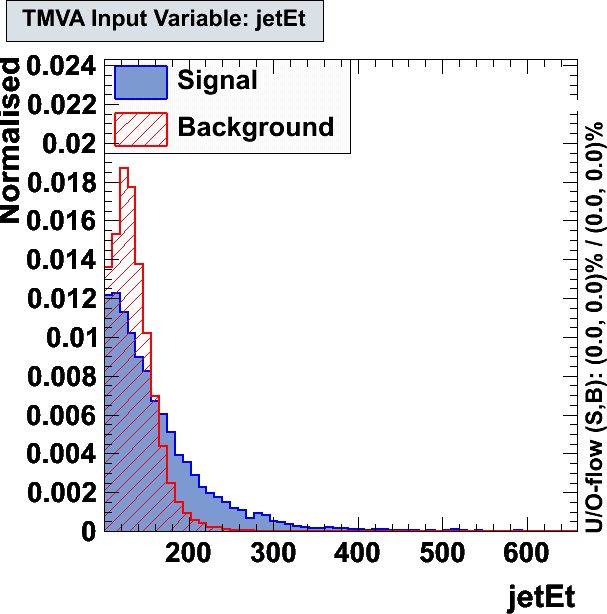
\includegraphics[width=1.0\textwidth]{images/jetet.png}
\end{minipage}
 \hfill
\begin{minipage}{5.5cm}
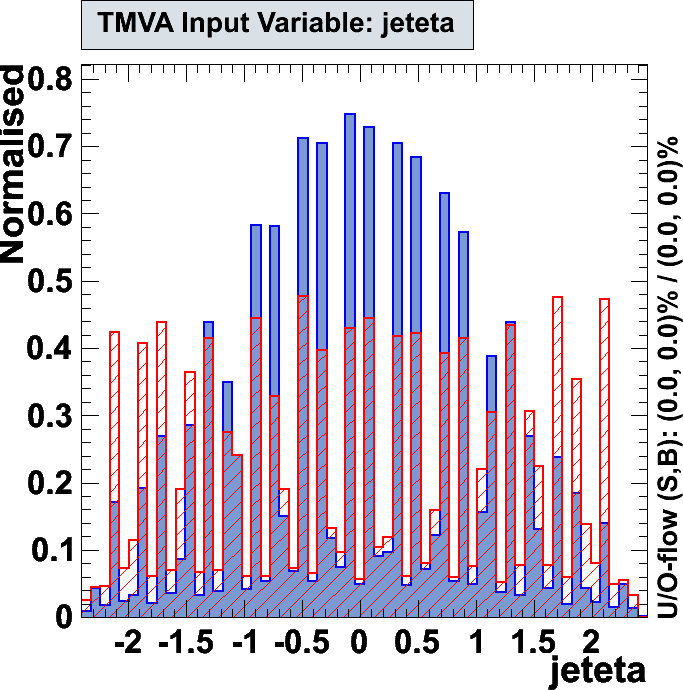
\includegraphics[width=1.0\textwidth]{images/jeteta.png}
\end{minipage}
%\begin{minipage}{3.0cm}

Example of data used in $\tau$ tagging. \\Left: Jet $E_T$ ({\tt jetEt}) variable, Right: Jet $\eta$ ({\tt jeteta}).
%\end{minipage}
\label{fig:variables}
\end{figure}


}

\bibliographystyle{alpha}  % Options plain, unsrt, alpha, abbrv
\bibliography{chep09} %10 p

\end{document}

\fi %slides



